\documentclass{article}
\usepackage[numbers]{natbib}
\usepackage{booktabs}
\usepackage{multirow}
\usepackage{amsmath}
\usepackage{hyperref}
\usepackage{overpic}
\usepackage{amssymb}
\usepackage{epigraph}
\usepackage[accepted]{dlaiml2026}

\usepackage{graphicx}

%%% STUDENTS: FILL IN WITH YOUR OWN INFORMATION
\dlaititlerunning{Solidity Code Synthesizer with LLMs and Partial Model Checking}

\begin{document}

\twocolumn[
	%%% STUDENTS: FILL IN WITH YOUR OWN INFORMATION
	\dlaititle{Solidity Code Synthesizer with LLMs and Partial Model Checking}

	\begin{center}\today\end{center}

	\begin{dlaiauthorlist}
		\dlaiauthor{Luca Sforza}{}
		\dlaiauthor{Roberto Di Rosa}{}
	\end{dlaiauthorlist}
	%%% STUDENTS: FILL IN WITH YOUR OWN INFORMATION
	\dlaicorrespondingauthor{Luca Sforza}{sforza.2050030@studenti.uniroma1.it}
	\dlaicorrespondingauthor{Roberto Di Rosa}{dirosa.2043388@studenti.uniroma1.it}

	\vskip 0.3in
]


\printAffiliationsAndNotice{}

\epigraph{Program testing can be used to show the presence of bugs, but never to show their absence!}
{\textit{― Edsger W. Dijkstra }}

\begin{abstract}
	%
	This is a \LaTeX template for writing your project report, to be submitted as part of the final exam. The template can not be modified (you can not change margins, spaces, etc.), and using this template is mandatory. Please read the main text for further details.
	%
\end{abstract}

\section{Introduction}

In questo lavoro vogliamo presentare un algoritmo per la sintesi
di codice per lo sviluppo di applicazioni nella blockchain.

\section{State of Art}
This not a new problem, others have thought about solving it.
Google tried a Methodology similar to ours \cite{austin2021program} this gave us the concept of overageneralization, overfitting of the invariants and others.
But the main limitation is that they do not try to optimize the generated code which we actually do.
We could not find others who tried to do the same thing as ours they usually tried something much simpler \cite{ye2025bridging} \cite{devito2025llm} which tries to fix compilation problems.
Others have tried to use LLMs to search for security vulnerabilities \cite{le2024robust}.
Here \cite{chen2026solagent} they tried to make a framework for the same purpouse as ours, but the testing is lacking since they seem to use only unit testing.
Some have tried to use LLMs to "verify" the generated code \cite{bartoletti2026llms} but as they admit in their paper, 
it's not a substitution of formal or even fuzzy testing.

\section{Methodology}
\subsection{Our Approach to Software Engineering}
In the world of software engineering we model the process of building a program as show in  figure \ref{img:sdc}.
\begin{figure}[h]
  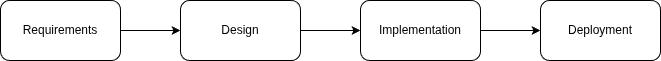
\includegraphics[width=0.5 \textwidth]{software_cicle.drawio.png}
	\caption{Software Development Cycle}
  \label{img:sdc}
\end{figure}
We aim to automate only the implementation phase, all of the other phases are handled by humans.
The kind of implementation we want to automate is TDD(Test-Driven-Development), but we heavily discourage the usage of Unit Tests.
The main reason is that unit tests do not prove that the candidate program works for any state of the system i.e. for any possible input.
So we used Partial Model Checking via Smt solvers, the tests are the definition of invariants of the system which must not be broken, the role of the smt solver 
is to prove that the invariants we defined hold for all of the possible states in the system.

\begin{equation}
	S = \{s \mid s \text{ is a constraint in some type of logic } \}
\end{equation}

\begin{equation}
	A = \{\pi \mid  \forall s \in S \implies \pi \models s\}
\end{equation}
Formally in the design phase we defined a set of constraints $\textbf{S}$ and $\textbf{A}$ the set of all possible programs which model our system, 
this is called model checking.
But we relaxed the definition of A permitting programs for which it is not feasible to prove their correctness for every possible state, 
therefore we are actually doing partial model checking.

\subsection{Workflow implementation}
\begin{figure}[h]
  \centering
  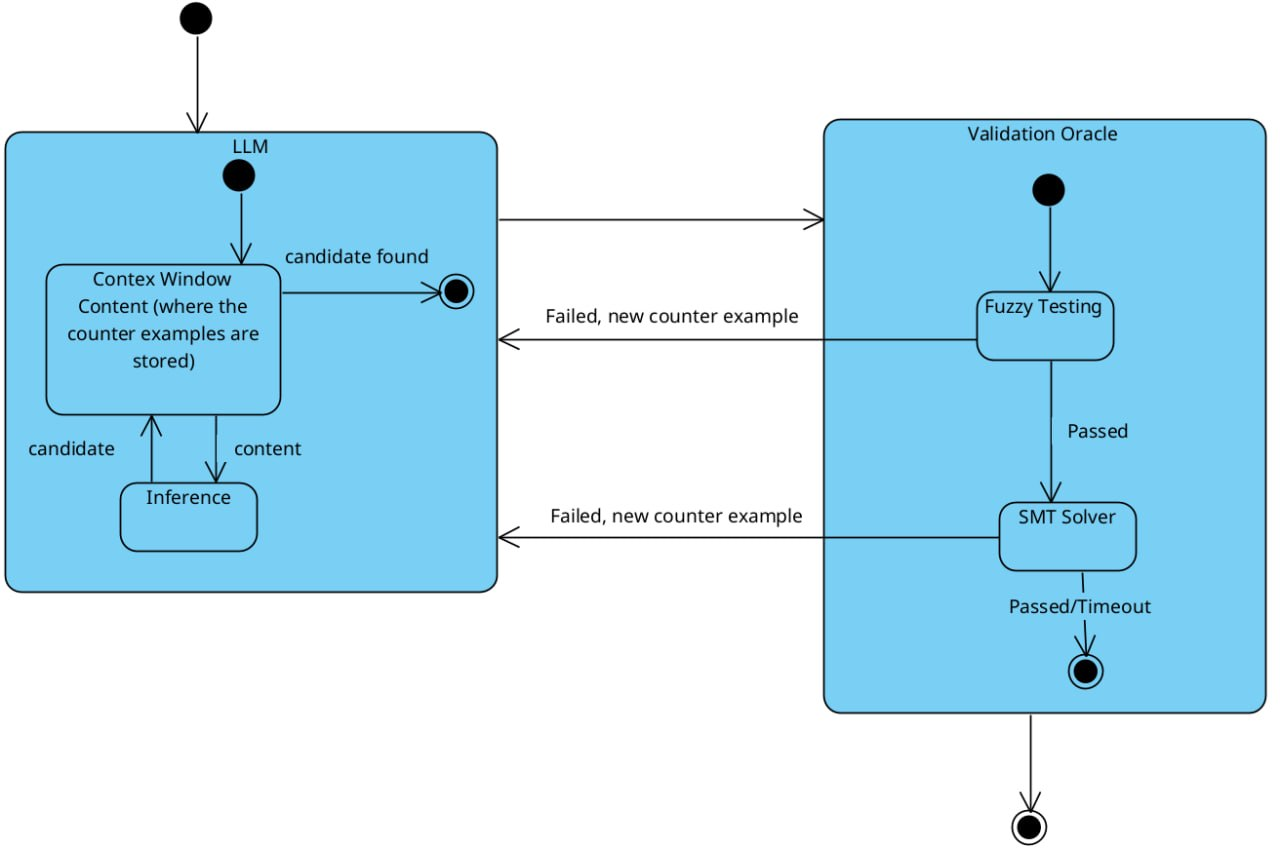
\includegraphics[width=0.35 \textwidth]{project/synthLoop.jpg}
  \caption{Synthesis loop}
  \label{img:sl}
\end{figure}
We implemented this idea by following the example of \cite{david2017program}:
\begin{enumerate}
  \item Synthesis by sketch \cite{david2017program} done in the following manner, the Analyst/Designer formalizes the User requests \footnote{i.e. UML,ER,FOL,SOL}.
These formalizations are then transformed into the skeleton of the project via a deterministic code generator.
The analyst does this to diminish the search space of all possible programs, the LLM completes the skeleton.
  \item Synthesis by Counter Example \cite{david2017program} as shown in this Figure \ref{img:sl} The LLM proposes a  program which is then checked by the smt solver, if the solver finds a counter-example the
LLM continues the generator loop.
We optimized this by adding a fuzzy testing \footnote{https://www.blackduck.com/glossary/what-is-fuzz-testing.html} phase which allows us to skip the SMT if the fuzzy tester fails.
\end{enumerate}
LLMs by nature are non deterministic \footnote{This can vary if we change some Hyperparameter e.g. temperature}, therefore we need to constrain them to follow the workflow.
We do this by following the Hook \footnote{https://code.claude.com/docs/en/hooks} and MCP tools \footnote{https://modelcontextprotocol.io/docs/getting-started/intro}.
The implemented hooks are triggered at:
 \begin{enumerate}
   \item PreToolUse: Is used to make the model only edit the files we want to be modified \footnote{For example we do not want the model to change the invariants, etc...}.
   \item PostToolUse: Is used to assure that the model does not modify the skeleton of the application\footnote{e.g. Changing the signature of functions, etc...}.
   \item Stop: Is used to guarantee a final state for the model checking, so SMT solver must either succeed or timeout othewise the LLM must continue with the generation of candidates.
 \end{enumerate}

We also developed an MCP server which exposes different tools to the model which allow the model to compile,do only fuzzy testing and to propose a candidate for complete testing.
The MCP tool gives back the counter-example if necessary.
\subsection{Why Blockchains?}
There are some technical reasons: we can easily tell which implementation is better than the others.
% \begin{equation}
%   \exists \bold{P}  \forall x 
% \label{eq:}
% \end{equation}
\begin{gather*}
\text{Let } \mathcal{D}_\pi \text{ gas distribution of } \pi \text{ on fuzzy input.} \\
\psi(p) = \operatorname{Median}(\mathcal{D}_\pi) = \inf\{g \in \mathbb{N} : F_\pi(g) \ge 1/2\},\\ 
\quad F_\pi(g) = \Pr_{X \sim \mathcal{D}_\pi}(X \le g). \\
 \hat{\psi}_n(p) = \operatorname{Median}\bigl(\operatorname{gas}(p, x_i) : i=1,\dots,n\bigr) , x_i \overset{\text{i.i.d.}}{\sim} \mathcal{D}_\pi. \\
\text{Objective: } \pi^* = \arg\min_{\pi \in A} \hat{ \psi }_n(\pi). \\
\label{eq:gascost}
\end{gather*}
We do this by measuring the median of the GAS \footnote{https://ethereum.org/gas/} usage of the program this metric is given by fuzzy testing as seen in \ref{eq:gascost}.
This does not find us the real minimum, we are solving a black box problem since we cannot know the real $\psi$, 
we use the random search algorithm to find possible candidates which will fill our gas cost distribution function.
This means that the LLM will try different approaches\footnote{i.e. We give the llm different seeds} to see the most optimal one for the number of runs we made.

\section{Evaluation}

\section{Conclusion}

% Cose da spiegare
% Cos'è il program synthesiz, citare paper program_synthesiz.pdf
%   - Spiegare programazzione automatica per contro esempio e by skect, che poi è quello che utilizziamo
% Introdurre lo state-of-art e spiegare i problemi tipici della sintesi con LLM, papaer llm_synthesiz.pdf
% Spiegare anche lavoro specifico fatto per la blockchain


% Metodologia
% Spiegare ciclo sviluppo del software per motivare la nostra Metodologia:
% La nostra Metodologia è generare deterministicamente codice dato un UML e
% i test sono scritti da umani. Teoricamente i test si potrebbero generare deterministicamente
% usando la logica del primo ordine/ Modale usando una DSL (Domain Specific Language), ma questo
% va al di fuori dello scopo di questo progetto, quindi sono stati presi test stock.
%
% Spiegare algoritmo di sintesi tramite hook e tool come claude code.
%
% Spiegare come abbiamo usato gli MCP server per la compilazione, il testing e raccolta dei dati sperimentali
%

% Test sperimentali dove si mette a confronto Qwen 3.6 finetunato su solidity Qwen Next Coder generico e Deep Seek v-4
% sui progetti: Auction, ERC4626, terzo progetto prendere uno grande
%
% Dei plot serve: % di errori di compilazione, Numero di volte in cui la sintesi è fallita, % di invarianti dimostrate, gas efficiency
%

% Conclusioni: descrizione dei risultati, commenti sui sviluppi dei modelli locali.

\bibliographystyle{abbrvnat}
\bibliography{references}

\end{document}

